% Licence, CC-BY
% This template borrowed from Karthik Ram, for Berkeley-ifcation of the Amsterdam theme.
\documentclass[serif]{beamer}
\usepackage{graphicx}
\usepackage{color}
\usepackage{xcolor}

%% maxwidth is the original width if it is less than linewidth
%% otherwise use linewidth (to make sure the graphics do not exceed the margin)

\makeatletter
\def\maxwidth{ %
  \ifdim\Gin@nat@width>\linewidth
    \linewidth
  \else
    \Gin@nat@width
  \fi
}
\makeatother

\definecolor{fgcolor}{rgb}{0.345, 0.345, 0.345}
\newcommand{\hlnum}[1]{\textcolor[rgb]{0.686,0.059,0.569}{#1}}%
\newcommand{\hlstr}[1]{\textcolor[rgb]{0.192,0.494,0.8}{#1}}%
\newcommand{\hlcom}[1]{\textcolor[rgb]{0.678,0.584,0.686}{\textit{#1}}}%
\newcommand{\hlopt}[1]{\textcolor[rgb]{0,0,0}{#1}}%
\newcommand{\hlstd}[1]{\textcolor[rgb]{0.345,0.345,0.345}{#1}}%
\newcommand{\hlkwa}[1]{\textcolor[rgb]{0.161,0.373,0.58}{\textbf{#1}}}%
\newcommand{\hlkwb}[1]{\textcolor[rgb]{0.69,0.353,0.396}{#1}}%
\newcommand{\hlkwc}[1]{\textcolor[rgb]{0.333,0.667,0.333}{#1}}%
\newcommand{\hlkwd}[1]{\textcolor[rgb]{0.737,0.353,0.396}{\textbf{#1}}}%

\definecolor{shadecolor}{rgb}{.97, .97, .97}
\definecolor{messagecolor}{rgb}{0, 0, 0}
\definecolor{warningcolor}{rgb}{1, 0, 1}
\definecolor{errorcolor}{rgb}{1, 0, 0}

\setbeamertemplate{frametitle}[default][center]
\setcounter{secnumdepth}{-1}
\usetheme{Amsterdam}

%% Get a pagenumber?
\expandafter\def\expandafter\insertshorttitle\expandafter{%
  \insertshorttitle\hfill%
  \insertframenumber\,/\,\inserttotalframenumber}

\usepackage{tikz}

% --------------------------------------------------------------


% --------------------------------------------------------------
% code syntax highlighting for xml
\usepackage{listings}

\usepackage{color}
\definecolor{gray}{rgb}{0.4,0.4,0.4}
\definecolor{darkblue}{rgb}{0.0,0.0,0.6}
\definecolor{cyan}{rgb}{0.0,0.6,0.6}

\lstset{
  basicstyle=\tiny\ttfamily,
  columns=fullflexible,
  showstringspaces=false,
  commentstyle=\color{gray}\upshape
}

\lstdefinelanguage{XML}
{
  morestring=[b]",
  morestring=[s]{>}{<},
  morecomment=[s]{<?}{?>},
  stringstyle=\color{black},
  identifierstyle=\color{darkblue},
  keywordstyle=\color{cyan},
  morekeywords={xmlns,version,type}% list your attributes here
}

\lstset{language=XML}
% --------------------------------------------------------------

% Those icons  in the references are terrible looking.
\setbeamertemplate{bibliography item}[text]


\title{Module development for FCO analysis}
\author[Kathryn D. Huff]{
\includegraphics[height=2cm]{bk}\\Kathryn D. Huff}
\begin{document}
\maketitle

%%--------------------------------%%

\section{Background}

% --------------------------------------------------------------
\begin{frame}[fragile]
  \frametitle{Scenario Definition}
A transition scenario which starts with the current once-through LWR fuel cycle, and moves toward a fleet of SFRs with 100\% recycle of spent fuel. 
\begin{itemize}
\item Simulation lasts until transition to 100\% SFRs is complete. 
\item Installed capacity is constant (100GWe).  
\item The transition is driven by availability of SFR fuel.
\end{itemize}

Specifically, when sufficient separated material is present, an LWR ($1000$MWe) should be decommissioned and replaced with three ($333.\bar{3}$) SFRs.

\end{frame}
% --------------------------------------------------------------
\begin{frame}[fragile]
  \frametitle{Desired Outputs}
The desired outputs of this simulation include 
\begin{itemize}
\item deployment metrics (i.e., the year during which the transition becomes complete). 
\item installed capacity profiles should demonstrate that generating shortages do not occur
\item material metrics such as separated surplus PU or TRU profiles, 
\item LWR used fuel reprocessing rate (t/yr), 
\item SFR used fuel reprocessing rate (t/yr),  
\item LWR used fuel mass in storage (t), 
\item and SFR used fuel mass in storage (t).
\end{itemize}
\end{frame}
% --------------------------------------------------------------
\begin{frame}[fragile]
  \frametitle{Scenario Definition}
\footnotesize{
\begin{table}[htbp]
\centering
\begin{tabular}{|l|l|l|}
\hline
Commodity  &     Offered By  &    Requested By \\
\hline
Natural  U & Mine & Enrichment \\
LEU & Enrichment & LWRFuelFab \\
Depleted U & Enrichment & SFRFuelFab \\
fresh LWR fuel & LWRFuelFab & LWR \\
fresh SFR fuel & SFRFuelFab & SFR \\
LWR UNF & LWR & LWRWetStorage \\
SFR UNF & SFR & SFRWetStorage \\
cool LWR UNF & LWRWetStorage & LWRSeparation \\
cool SFR UNF & SFRWetStorage & SFRSeparation \\
separated LWR U & LWRSeparation & SFRFuelFab \\
separated LWR TRU & LWRSeparation & SFRFuelFab \\
separated SFR U & SFRSeparation & SFRFuelFab \\
separated SFR TRU & SFRSeparation & SFRFuelFab \\
\hline
\end{tabular}
\caption{Commodity flow in the transition simulation}
\label{tab:commods}
\end{table}
}
\end{frame}

% --------------------------------------------------------------
\begin{frame}[fragile]
  \frametitle{Scenario Definition}
\begin{figure}[htpb]
\begin{center}
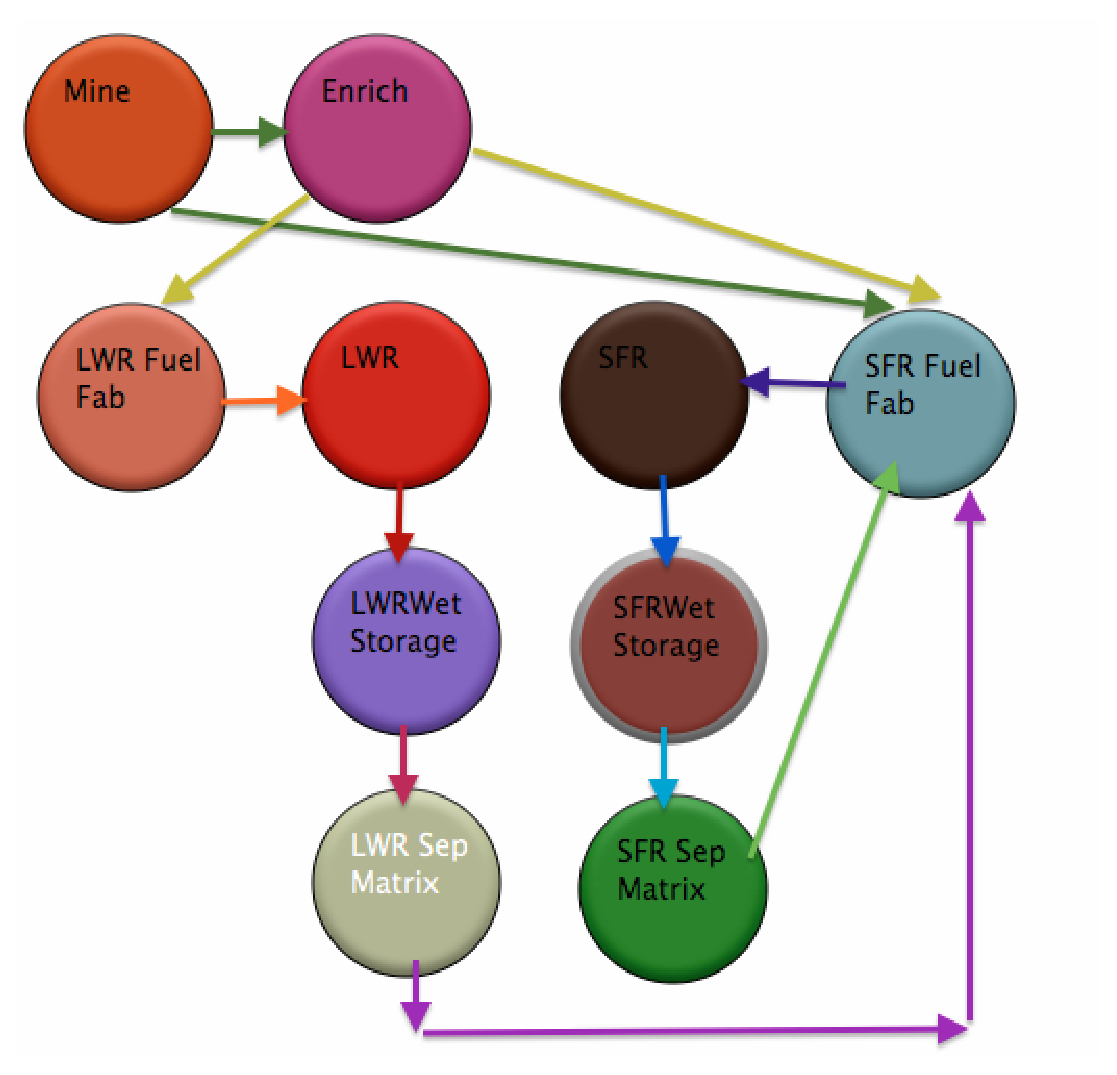
\includegraphics[width=0.4\textwidth]{cycic_img.eps}
\end{center}
\caption{Image generated by Cycic
\cite{flanagan_input_2013}
, the input controller for Cyclus
\cite{carlsen_cyclus_2014}.} 
\label{fig:cycic_img}
\end{figure}
\end{frame}
% --------------------------------------------------------------
\begin{frame}[fragile]
\footnotesize{
\begin{table}
\centering
\begin{tabular}{|l|l|r|}
\hline
\textbf{Facility Type} &\textbf{Agent} & \textbf{Key Parameters}\\
\hline
Mine & SourceFacility & Capacity\\
\hline
Enrichment & EnrichmentFacility & feed enrchment\% \\
& & tails enrichment\% \\
& & Process time \\
\hline
LWRFuelFab & StreamBlender & Process time\\
& & Fissile Source\\
\hline
SFRFuelFab & StreamBlender  & Process time\\
& & Fissile Sources\\
& & Fertile Sources\\
\hline
LWR & BatchReactor & Capacity \\
& & Batches per core \\
& & Cycle length\\
& & In/Out Recipes \\
\hline
SFR & BatchReactor & Capacity\\
& & Batches per core \\
& & Cycle length\\
& & In/Out Recipes \\
\hline
LWRWetStorage & CommodConverter & Process time\\
\hline
SFRWetStorage & CommodConverter & Process time\\
\hline
LWRSeparation & SeparationMatrix & Capacity\\
& & Process Time\\
& & Efficiency Matrix\\
\hline
SFRSeparation & SeparationMatrix & Capacity\\
& & Process Time\\
& & Efficiency Matrix\\
\hline
HLW Repository & SinkFacility & Capacity \\
\hline
\end{tabular}
\caption{Facilities and their implementations with key parameters.}
\label{tab:facimpl}
\end{table}
}
\end{frame}

\input{timeline}
\section{Basics}



% --------------------------------------------------------------
\begin{frame}[fragile]
  \frametitle{Available Archetypes}
  Cycamore has many available archetypes \cite{carlsen_cycamore_2014}.
  \begin{itemize}
\item The \textbf{GrowthRegion} archetype maintains a power generation profile specified by the user. 
\item The reactors can be represented by the existing \textbf{BatchReactor} 
facility archetype.
\item The Mine and Repository can be represented by the \textbf{Source} and 
\textbf{Sink}.
\item The Enrichment Facility can be represented by the \textbf{EnrichmentFacility}
\end{itemize}
\end{frame}

% --------------------------------------------------------------
\begin{frame}[fragile]
  \frametitle{Available Archetypes : Easy Access}
\footnotesize{
\begin{lstlisting}
  <archetypes>
    <spec>
      <lib>cycamore</lib><name>Source</name>
    </spec>
    <spec>
      <lib>cycamore</lib><name>EnrichmentFacility</name>
    </spec>
    <spec>
      <lib>cycamore</lib><name>GrowthRegion</name>
    </spec>
    <spec>
      <lib>cycamore</lib><name>BatchReactor</name>
    </spec>
    <spec>
      <lib>cycamore</lib><name>Sink</name>
    </spec>
\end{lstlisting}
\ldots
}
\end{frame}

% --------------------------------------------------------------
\begin{frame}[fragile]
  \frametitle{Available Region}
\footnotesize{
  \begin{lstlisting}
  <region>
    <name>SingleRegion</name>
    <config>
      <GrowthRegion>
        <commodity_name>power</commodity_name>
        <demand_types>
          <val>linear</val>
        </demand_types>
        <demand_params>
          <val>0 90</val> <!-- slope intercept -->
        </demand_params>
        <demand_times>
          <val>1</val>
        </demand_times>
      </GrowthRegion>
    </config>
    <institution>
\end{lstlisting}
}
\end{frame}
% --------------------------------------------------------------
\begin{frame}[fragile]
  \frametitle{Available Source and Sink}
  \begin{lstlisting}
  <facility>
    <name>Mine</name>
    <lifetime>1200</lifetime>
    <config>
      <Source>
        <out_commod>nat_u</out_commod>
        <recipe_name>nat_u_recipe</recipe_name>
        <capacity>200000</capacity>
      </Source>
    </config>
  </facility>
\end{lstlisting}
\end{frame} 
% --------------------------------------------------------------
\begin{frame}[fragile]
  \frametitle{Available Reactors}
  \lstset{basicstyle=\tiny\ttfamily}
\begin{lstlisting}
  <facility>
    <name>LWR</name>
    <lifetime>1200</lifetime>
    <config>
      <BatchReactor>
        <fuel>
         <incommodity>fresh_lwr_fuel</incommodity>
         <inrecipe>fresh_lwr_fuel_recipe</inrecipe>
         <outcommodity>lwr_unf</outcommodity>
         <outrecipe>lwr_unf_recipe</outrecipe>
        </fuel>
        <processtime>12</processtime>
        <nbatches>9</nbatches> 
        <batchsize>9950.0</batchsize> 
        <nreload>2</nreload> 
        <commodity_production>
          <commodity>power</commodity>
          <capacity>90</capacity>
          <cost>90</cost>
        </commodity_production>
      </BatchReactor>
    </config>
  </facility>
\end{lstlisting}
\end{frame}



\section{New Archetypes}
\subsection{Commodity Converter Facility}

One versatile facility model contributed by this work is a simple 
representation of timed storage. After recieving material, this facility 
waits for a user-defined time period. Once that time period has passed, the 
material object is offered up as a new commodity type. 

In the case of a storage facility, for example, this model requests a commodity 
such as spent fuel, then waits for a cooling period before offering the same 
material as cooled spent fuel.

\begin{table}[h!]
\centering
\begin{tabular}{|l|r|r|r|}
\hline
\textbf{Parameter} & \textbf{Units} & \textbf{Default} & \textbf{Range}\\
\hline
Input Commodity& string & ``'' & any string\\
Output Commodity& string & ``'' & any string\\
Delay Time & months & $0$ & $0-\infty$\\
Storage Capacity & kg & \infty &$0-\infty$ \\
\hline
\end{tabular}
\caption{Input parameters for the Commodity Converter Facility Model}
\label{tab:commodconverter}
\end{table}


% --------------------------------------------------------------
\begin{frame}[fragile]
  \frametitle{Stream Blender} 
The process specified for SFR fuel fabrication from separated materials streams
can most concisely be described as blending into a recipe.
\begin{figure}[htbp!]
\begin{center}
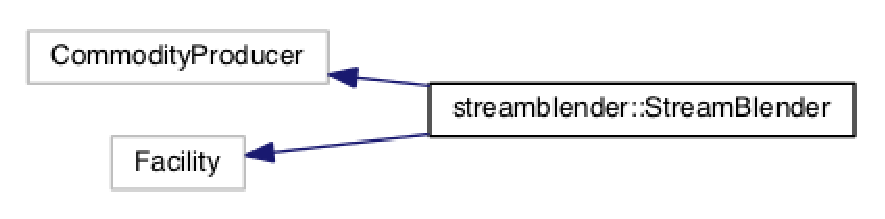
\includegraphics[width=0.8\textwidth]{sb_inherit}
\end{center}
\caption{Utilizes interfaces defined in Cyclus.}
\label{fig:sb_inherit}
\end{figure}
\end{frame}
% --------------------------------------------------------------
\begin{frame}[fragile]
  \frametitle{Stream Blender}
This new StreamBlender Facility Agent 
(\url{https://katyhuff.github.io/StreamBlender}) 
\cite{huff_market_2014} handles the combination of various commodity streams in 
appropriate proportions to achieve a goal recipe.  

\begin{itemize}
\item incoming commodities
\item incoming recipes
\item outgoing commodity
\item goal recipe
\item driving isotopes and sources
\item waste commodity (default = ''waste``)
\item process time (default = 0)
\end{itemize}
\end{frame}
% --------------------------------------------------------------
\begin{frame}[fragile]
\footnotesize{
\begin{lstlisting}
  <facility>
    <name>SFRFuelFab</name>
    <lifetime>1200</lifetime>
    <config>
      <StreamBlender>
        <in_commods>
          <val>rep_sfr_tru</val>
          <val>rep_lwr_tru</val>
          <val>rep_sfr_u</val>
          <val>dep_u</val>
          <val>nat_u</val>
        </in_commods>
        <out_commod>fresh_sfr_fuel</out_commod>
        <out_recipe>fresh_sfr_fuel_recipe</out_recipe>
        <in_recipes>
          <val>rep_sfr_tru_recipe</val>
          <val>rep_lwr_tru_recipe</val>
          <val>rep_sfr_u_recipe</val>
          <val>dep_u_recipe</val>
          <val>nat_u_recipe</val>
        </in_recipes>
\end{lstlisting}
}
\end{frame}
% --------------------------------------------------------------
\begin{frame}[fragile]
\footnotesize{
\begin{lstlisting}
        <isos>
          <val>94240</val>
          <val>94240</val>
          <val>92235</val>
          <val>92235</val>
          <val>92235</val>
          <val>94239</val>
          <val>95241</val>
        </isos>
        <sources>
          <val>rep_sfr_tru</val>
          <val>rep_lwr_tru</val>
          <val>rep_sfr_u</val>
          <val>dep_u</val>
          <val>nat_u</val>
          <val>rep_lwr_tru</val>
          <val>rep_lwr_tru</val>
        </sources>
        <process_time>12</process_time>
      </StreamBlender>
    </config>
  </facility>
\end{lstlisting}
}
\end{frame}

\subsection{Matrix-Based Separation Facility Model}

By describing the separations process as a simple matrix of efficiencies, a 
simple 1:N material stream transformation is conducted. The specific process 
chemistry for the separation at hand is treated as elemental, as representative 
of a non-laser separations process. The matrix of separation efficiencies has a 
default value: the identity matrix. In this context, the identity matrix 
represents complete and perfect elemental separation without losses. 

\begin{align}
  \left[
    \begin{array}{c c c c c c c}
      \eta_{11} & . & . & . & . & . & \eta_{1M} \\
      \eta_{21} & . & . & . & . & . & \eta_{2M} \\
      . & . & . & . & . & . & . \\
      . & . & . & . & . & . & . \\
      . & . & . & . & . & . & . \\
      \eta_{N1} & .  & . & . & . & . & \eta_{NM} \\
    \end{array}
    \right]
  \left[
    \begin{array}{c}
      I_1\\
      I_2\\
      . \\
      . \\
      . \\
      I_N\\
    \end{array}
    \right]
    =
    \left[
      \begin{array}{ c }
        E_1\\
        E_2\\
        .\\
        .\\
        .\\
        E_M\\
      \end{array}
      \right]
\label{defaultsep}
\end{align}

Thus, for realistic separations, the user is expected to produce an efficiency 
matrix representing the separations technology of interest to them. 
By requesting the feedstock from the 
appropriate markets, the facility acquires an unseparated feedstock stream. 
Based on the input parameters  in Table \ref{tab:sepmatrix}, the separations 
process proceeds within the timesteps and other constraints of the simulation. 


\begin{table}[h!]
\centering
\begin{tabular}{|l|r|r|r|}
\hline
\textbf{Parameter} & \textbf{Units} & \textbf{Default} & \textbf{Range}\\ 
\hline
& & & \\
\hline
\end{tabular}
\caption{Input parameters for the Matrix-Based Separation Facility Model}
\label{tab:sepmatrix}
\end{table}

Thereafter, separated streams as well as a stream of losses are offered the 
appropriate markets for consumption by other facilities. In the transition 
scenario at hand, the StreamBlender fuel fabridation facility purchases the 
streams it desires in order to produce SFR fuel. 


\subsection{Market Driven Institution}
\label{sec:mktdriveninst}
The new Institution Agent was based on an already existing institution
model, but required a market-driven deployment capability to
faithfully model this scenario. 

That is, by relying on inheritance from a mixin class already available within 
the \Cyclus toolkit, an institution can deploy and decommission facilities 
based on any decision criteria. By also relying on the dynamic resource 
exchange interface, it is possible to base that decision criteria on the 
availability of resources being offered by other facility agents in the 
simulation. 

In this case, a specific quantity of separated transuranic material must exist 
before an LWR can be decommissioned (to be replaced with three SFRs). That 
decision criteria, combined with the capability of decommissioning facilities, 
gives the Decommisioning Institution. 



\section{Future}
\input{out_formatting}
\input{personnel}

\begin{frame}[fragile]
\frametitle{Future}
All instructions and code for installing and running the code-to-code 
comparison are online : \url{https://github.com/katyhuff/transition} and a discussion is 
available in an ANS Winter 2014 summary \cite{huff_extensions_2014}.
\end{frame}


\begin{frame}[fragile]
\frametitle{Future}
\begin{itemize}
\item sqlite to csv (Russell Nibbelink) 
\item material movement and deployment debugging (Denia Djokic)
\item other FCO data scenarios (Harris Greenberg, Max Fratoni, etc.)
\end{itemize}
\end{frame}


This work was conducted <LLNL text>.

Additionally, this material is based upon work supported by the Department of 
Energy National Nuclear Security Administration under Award Number(s) 
DE-NA0000979. % Katy's appointment is NSSC, must acknowledge for everything

<disclaimer text>.


%%--------------------------------%%
%%--------------------------------%%
\begin{frame}[allowframebreaks]
  \frametitle{References}
  \bibliographystyle{ieeetr}
  {\footnotesize \bibliography{bibliography} }

\end{frame}

%%--------------------------------%%




\end{document}
